The wage gap is an oft-cited number that quantifies the difference between males and females in the economy: In the fourth quarter of 2016, white women earned 81.1\% as much as white men and African American women earned 92.1\% as much as African American men. This reveals a gap not only by gender, but also by race with African American women only earning 67.8\% as much as white men and African American men earning 73.6\% as much as white men.\footnote{\citet{USDPTL_2017_Wage_News-Release}.}

 Although this favors males, there are related measures of gender differences that favor females. In 2015, only 64 (103) per 100,000 (African American) females were incarcerated in comparison to 488 (2,613) per 100,000 (African American) males.\footnote{\citet{UDOJ_2016_PrisonersStatistics_Bulletin}.} Similarly, in 2012-2013, more females than males received bachelor's degrees across all races with large disparities for African Americans: 65\% of degrees conferred to African Americans were conferred to females.\footnote{\citet{UDOE_2016_Statistics_Report}.}

These differences are select measurements from the life-cycle trajectory of skill formation and labor market opportunities. Based on previous literature of skill formation, these later skills build on earlier skill development.\footnote{\citet{Cunha_Heckman_etal_2010_est_tech_cognoncog}.} Additionally, higher levels of these skills, especially social-emotional skills, can lead to more positive life-relevant outcomes like health.\footnote{\citet{Conti_etal_2016_LongTermHealth}.} The adult gender differences highlighted above can be the result of early-life differences that propagate over the life-cycle. We examine these differences by analyzing the effects of two nearly identical early childhood interventions. 

The interventions, the Carolina Abecedarian Project (ABC) and the Carolina Approach to Responsive Education (CARE), were randomized controlled trials using a sample of disadvantaged families in Chapel Hill, North Carolina with children born between 1972 and 1980. The treatment group received high-quality, intensive, early childhood education from birth until age 5. Researchers collected measures of cognitive, social-emotional, and parenting skills on the subjects in both the treatment and control groups during and after the intervention. 

Using the ABC/CARE sample and pooling across experimental groups, Figure~\ref{fig:intro-skills-plots} shows the skill differences between the males and females. Overall, there are few significant gender differences. Consistent with previous work, the females in the sample tend to perform better than the males in social-emotional and achievement skill measurements.\footnote{\citet{Baker-Milligan_2013_Boy-Girl-Differences}.} While the parents of males exhibit more positive parenting skills during later ages (3.5, 4.5, and 8 years), the parents of females exhibit more warmth and involvement.

\begin{sidewaysfigure}[H]
\begin{center}
\caption{Differences Between ABC/CARE Males and Females, Skill Measurements}
\label{fig:intro-skills-plots}
\begin{subfigure}[b]{0.49\textwidth}
	\caption{IQ Measurements}
	\label{fig:intro-skills-plots-cog}
	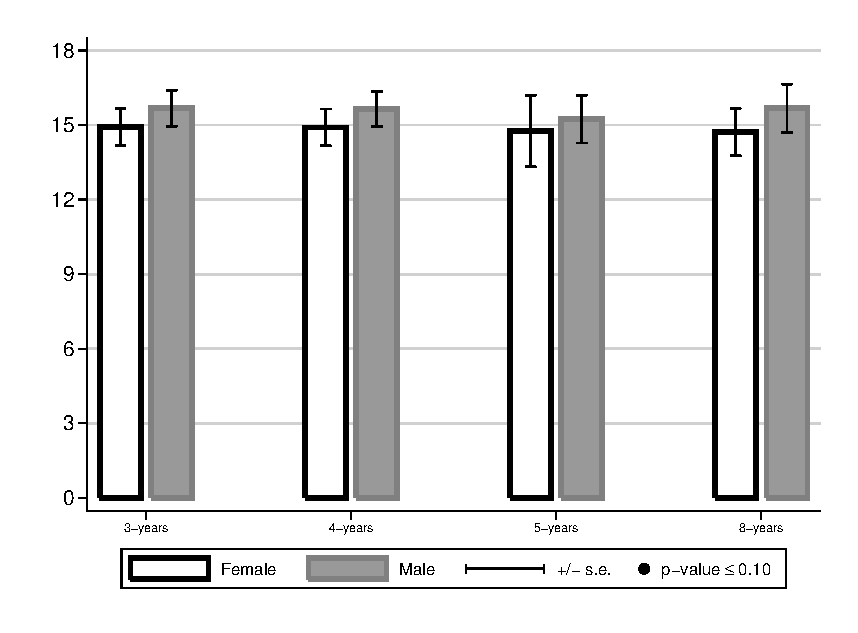
\includegraphics[width=\textwidth]{../output/abccare-gdiff-cog}
\end{subfigure}
\begin{subfigure}[b]{0.49\textwidth}
	\caption{Social-emotional Measurements}
	\label{fig:intro-skills-plots-ncog}
	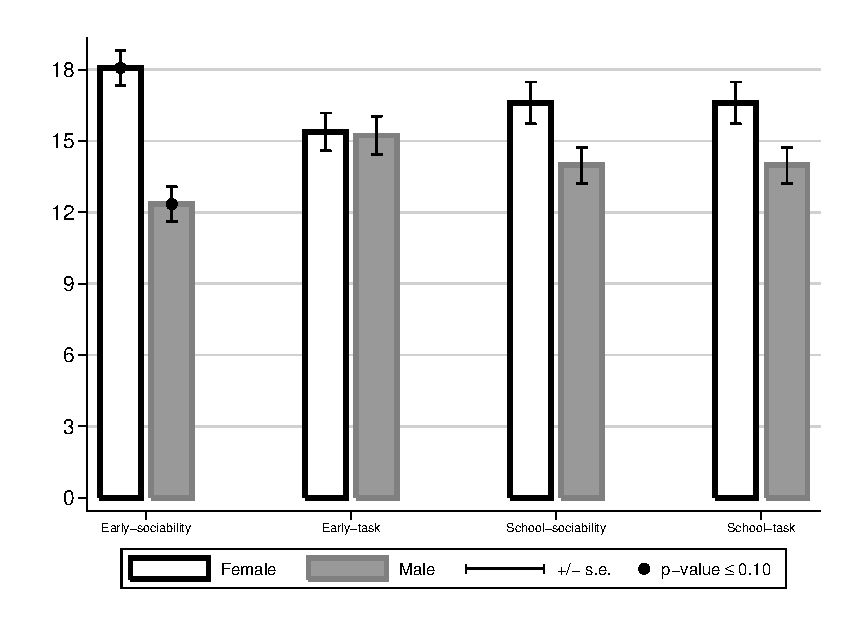
\includegraphics[width=\textwidth]{../output/abccare-gdiff-ncog}
\end{subfigure}

\begin{subfigure}[b]{0.49\textwidth}
	\caption{Achievement Measurements}
	\label{fig:intro-skills-plots-ach}
	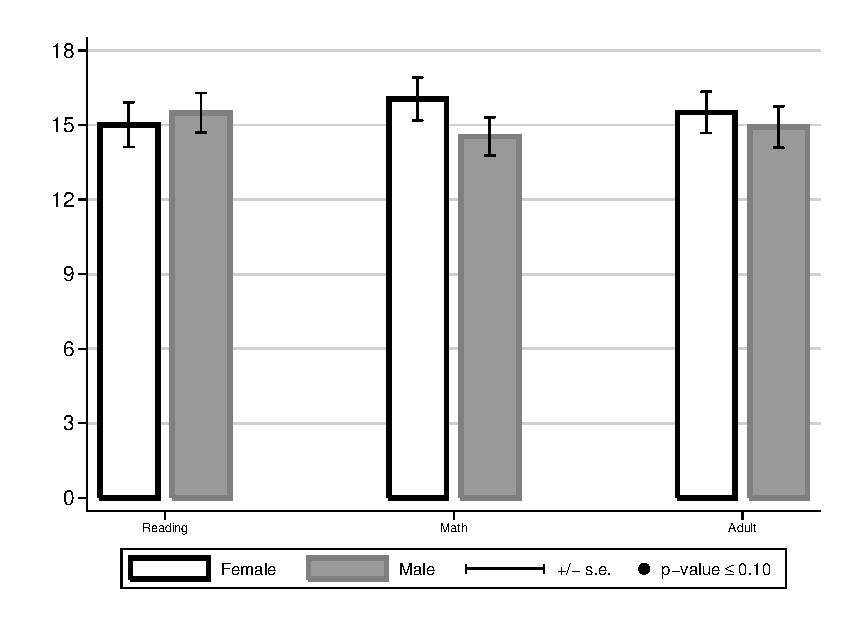
\includegraphics[width=\textwidth]{../output/abccare-gdiff-ach}
\end{subfigure}
\begin{subfigure}[b]{0.49\textwidth}
	\caption{Parenting Measurements}
	\label{fig:intro-skills-plots-parenting}
	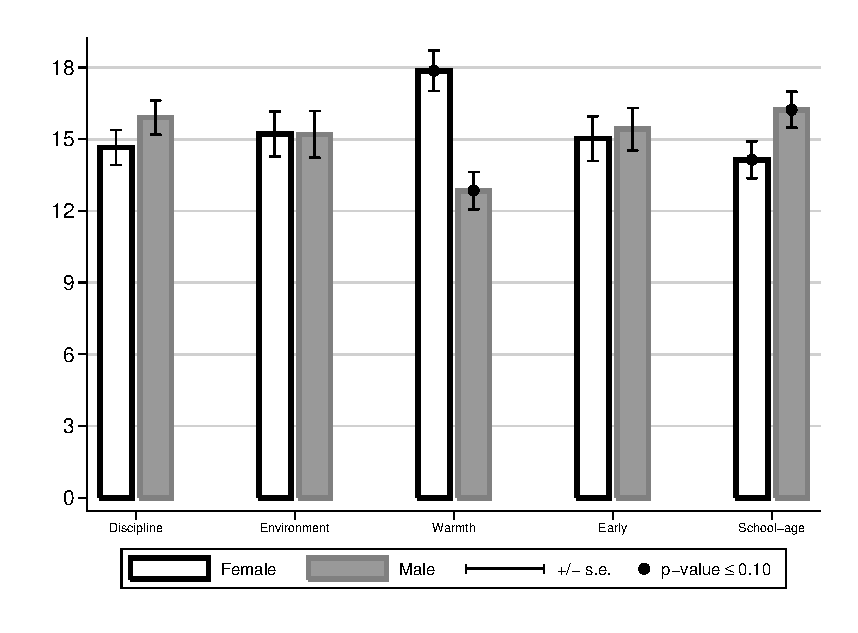
\includegraphics[width=\textwidth]{../output/abccare-gdiff-parenting}
\end{subfigure}
\end{center}
\raggedright \scriptsize
Note: These plots show the means of factor variables by gender, pooling across experimental groups. The capped lines show the standard errors and black points indicate that the female is significantly different than the males. These hypothesis tests are two-sided and computed using 200 bootstraps. All factor variables are calculated by principal factor analysis. The factors are then standardized and divided into 30 quantiles. The IQ factors include different measurements at the specified ages. The social-emotional factors are divided by early (0.5, 1, and 1.5 years) and school-age (6 and 8 years) variables. The scales presented here are sociability and task orientation. The achievement factors are school-age math and reading factors (6, 7.5, 8, 8.5, 9, and 12 years) and an adult factor combining math and reading at 21 years. The parenting factors include factors of the subscales absence of punishment (discipline), environmental factors (environment), and maternal warmth and involvement (warmth). The other factors combine these scales measured when the subjects were toddlers (0.5, 1.5, and 2.5 years) and when they were older (3.5, 4.5, and 8 years).
\end{sidewaysfigure}

We can also examine the gender differences in adult outcomes. Although females do better on average than males early in life, they lag behind males later in life in important outcomes. As shown in Figure~\ref{fig:intro-adult-outcomes}, females commit fewer crimes, but have worse health outcomes and lower education and income levels. 

\begin{figure}[H]
\begin{center}
\caption{Differences Between ABC/CARE Males and Females, Adult Outcomes}
\label{fig:intro-adult-outcomes}
	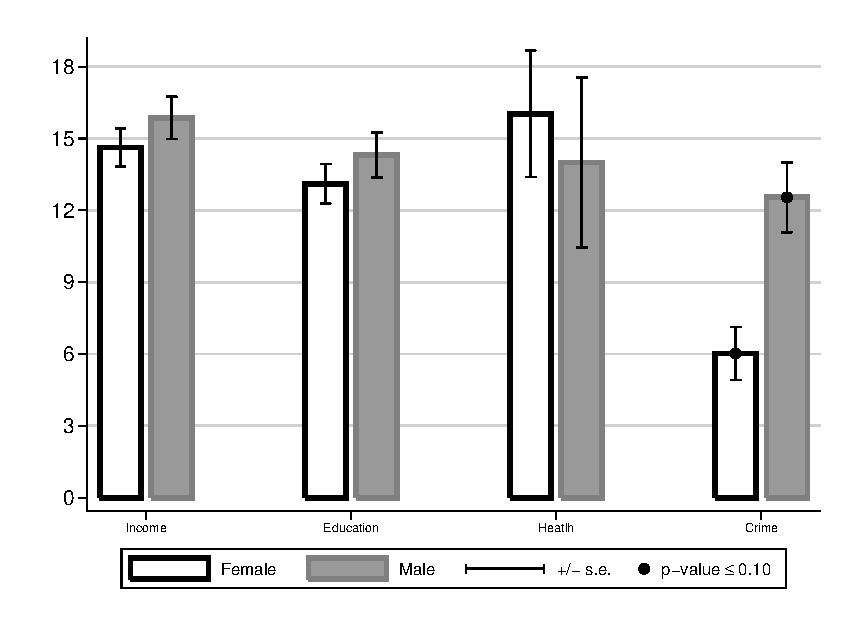
\includegraphics[width=0.9\textwidth]{../output/abccare-gdiff-adult}
\end{center}
\raggedright \scriptsize
Note: This plot shows the means of factor variables by gender, pooling across experimental groups. The capped lines show the standard errors and black points indicate that the female is significantly different than the males. These hypothesis tests are two-sided and computed using 200 bootstraps. All factor variables are calculated by principal factor analysis. The factors are then standardized and divided into 30 quantiles. The income factor is comprised of labor income at 21 and 30 years and employment at 30 years. The education factor is comprised of years of education and college graduation at 30 years and high school graduation at 21 years. The health factor is coded such that a higher value corresponds to socially undesirable outcomes. It is comprised of measures of drug and tobacco use, obesity, and hypertension. The crime factor is comprised of total felony and misdemeanor arrests using administrative data collected when the subjects were in their mid-30s.
\end{figure}

Although these mean differences do not include the effect of the early childhood education on improving these skills, many studies have shown the potential for early-life interventions to improve the skills of children, especially those from disadvantaged families.\footnote{\citet{Elango_Hojman_etal_2016_Early-Edu}.} Several of these studies separate analysis by gender and find that males and females benefit differently from early childhood education. For example, \citet{Heckman_Moon_etal_2010_QE} and \citet{Garcia_etal_2016_Comp_CBA_Unpublished}, both of which analyze randomized controlled trials with long-term data follow-ups, find that the intervention more positively affects education for females and labor market and health outcomes for males. Other studies analyzing programs with shorter-term data also find gender differences in early skills and academic outcomes.\footnote{\citet{Deming_2009_AEJAE} and \citet{Ou_Reynolds_2010_Mechanisms_CYSR} are examples of this.} 

We estimate the treatment effects by gender and find results consistent with these previous results. Although both males and females in the treatment group had reduced criminal activity, the crimes males in the sample tended to commit were less serious than those that the females tended to commit. Unlike in \citet{Garcia_etal_2016_Comp_CBA_Unpublished}, we do not weigh treatment effects by social cost. 

We compute standard treatment effects comparing the treatment and control group. This considers the treatment effect given that the families select the ``next best'' early childhood option for their child. This option can include staying at home with family or attending other center-based care of lower quality than the ABC/CARE intervention. We additionally compute treatment effects comparing the treatment group to the control group fixing those in the control group to these alternate counterfactuals. When fixing the control group to alternative preschool, the treatment effects tend to improve for males. In contrast, the treatment effects tend to improve for females when fixing the control group to staying at home. In order to summarize across the large number of variables, we present estimates from combining functions. Across all counterfactual scenarios, there were more positive treatment effects for females than for males. This is especially pronounced when fixing the control group to staying at home.

There are several explanations for the gender differences in the treatment effects. One explanation is that males are more fragile than females early in life, which would account for the early differences favoring females.\footnote{\citet{Schore_2017_IMHJ}.} Another explanation is that parents respond differently by gender while the children are developing and learning from center-based education and other sources of stimulation.\footnote{\citet{Baker-Milligan_2013_Boy-Girl-Differences}.} We explore the interaction of early childhood education with the gender of the child and parenting to help explain the gender differences of the treatment effects.

The paper proceeds as follows. We describe ABC/CARE in more detail in Section~\ref{sec:data}. We then discuss the parameters of interest in Section~\ref{sec:parameters} and describe our method for summarizing over the multitude of variables in Section~\ref{sec:combining-functions}. Section~\ref{sec:treatment-effects} displays the estimates of the parameters of interest and the combining functions. We discuss suggestive mechanisms through which the early-life skill differences mediate later-life gender differences in Section~\ref{sec:gender-differences}. Section~\ref{sec:conclusion} concludes.

%These gender results are variable across studies, however, obfuscating the conclusions.\footnote{\citet{Magnuson_Kelchen_Duncan_etal_2016_ECRQ} use effect sizes and program characteristics from 23 evaluations of early-life interventions to understand the association between program characteristics and effect sizes by gender. This meta-analysis finds that over the programs used, the most pronounced difference in treatment effects between males and females can be found for outcomes related to schooling, e.g. special education and grade retention. However, most of the programs do not have non-cognitive measures and the varied structure of the evaluations makes the conclusions for gender differences suggestive.} Even within the same program, different approaches to analyzing treatment effects can result in seemingly contradictory conclusions. Using data from the Carolina Abecedarian Project and the Carolina Approach to Responsive Education (ABC/CARE), \citet{Garcia_etal_2016_Comp_CBA_Unpublished} calculate a higher lifetime benefit-cost ratio for males (11.10) than for females (2.45), with these ratios including life-cycle projections of health, crime, and income. According to this analysis, the monetary returns of the program from a social perspective are driven more by males than females, making it appear that males benefit more from the program than do females. However, when looking at the treatment effects unweighted by monetary amounts, there are more positive treatment effects for females for certain categories (see Section~\ref{sec:gdiff}). Unlike the cost-benefit analysis, this aggregate result makes it appear that females benefit more from the program in skills, labor market outcomes, and crime outcomes. Although both of these measures aggregate across outcomes, they lead to seemingly contradictory conclusions on the differential effect of early childhood education.

%Understanding the mechanisms of the treatment effects complements the above analyses by explaining and understanding the later-life gender differences seen in both approaches. We address the contradiction by focusing on how early childhood education affects the skill formation process of males and females differently, with these skills in turn affecting other outcomes.\footnote{There is also evidence that the development of males and females differs at this age such that they experience early childhood interventions differently. See \citet{Beeghly-etal_2017_IMHJ,Dayton_2017_IMHJ,Iruka_2017_IMHJ,Schore_2017_IMHJ} for recent findings on the topic of different development of males and females early in life. We consider these findings complementary to our own.}

